%!TEX root = ../../../adrien_gomar_phd.tex

The mesh considered to compute this
CROR configuration is a single-blade passage meshed
with an O4H topology show in Fig.~\ref{fig:dream_mesh}. This is a classical
topology for turbomachinery computations that is here applied to 
a CROR.
\begin{figure}[htb]
  \centering
  \subfigure[Topology]{
    \label{fig:dream_mesh}
    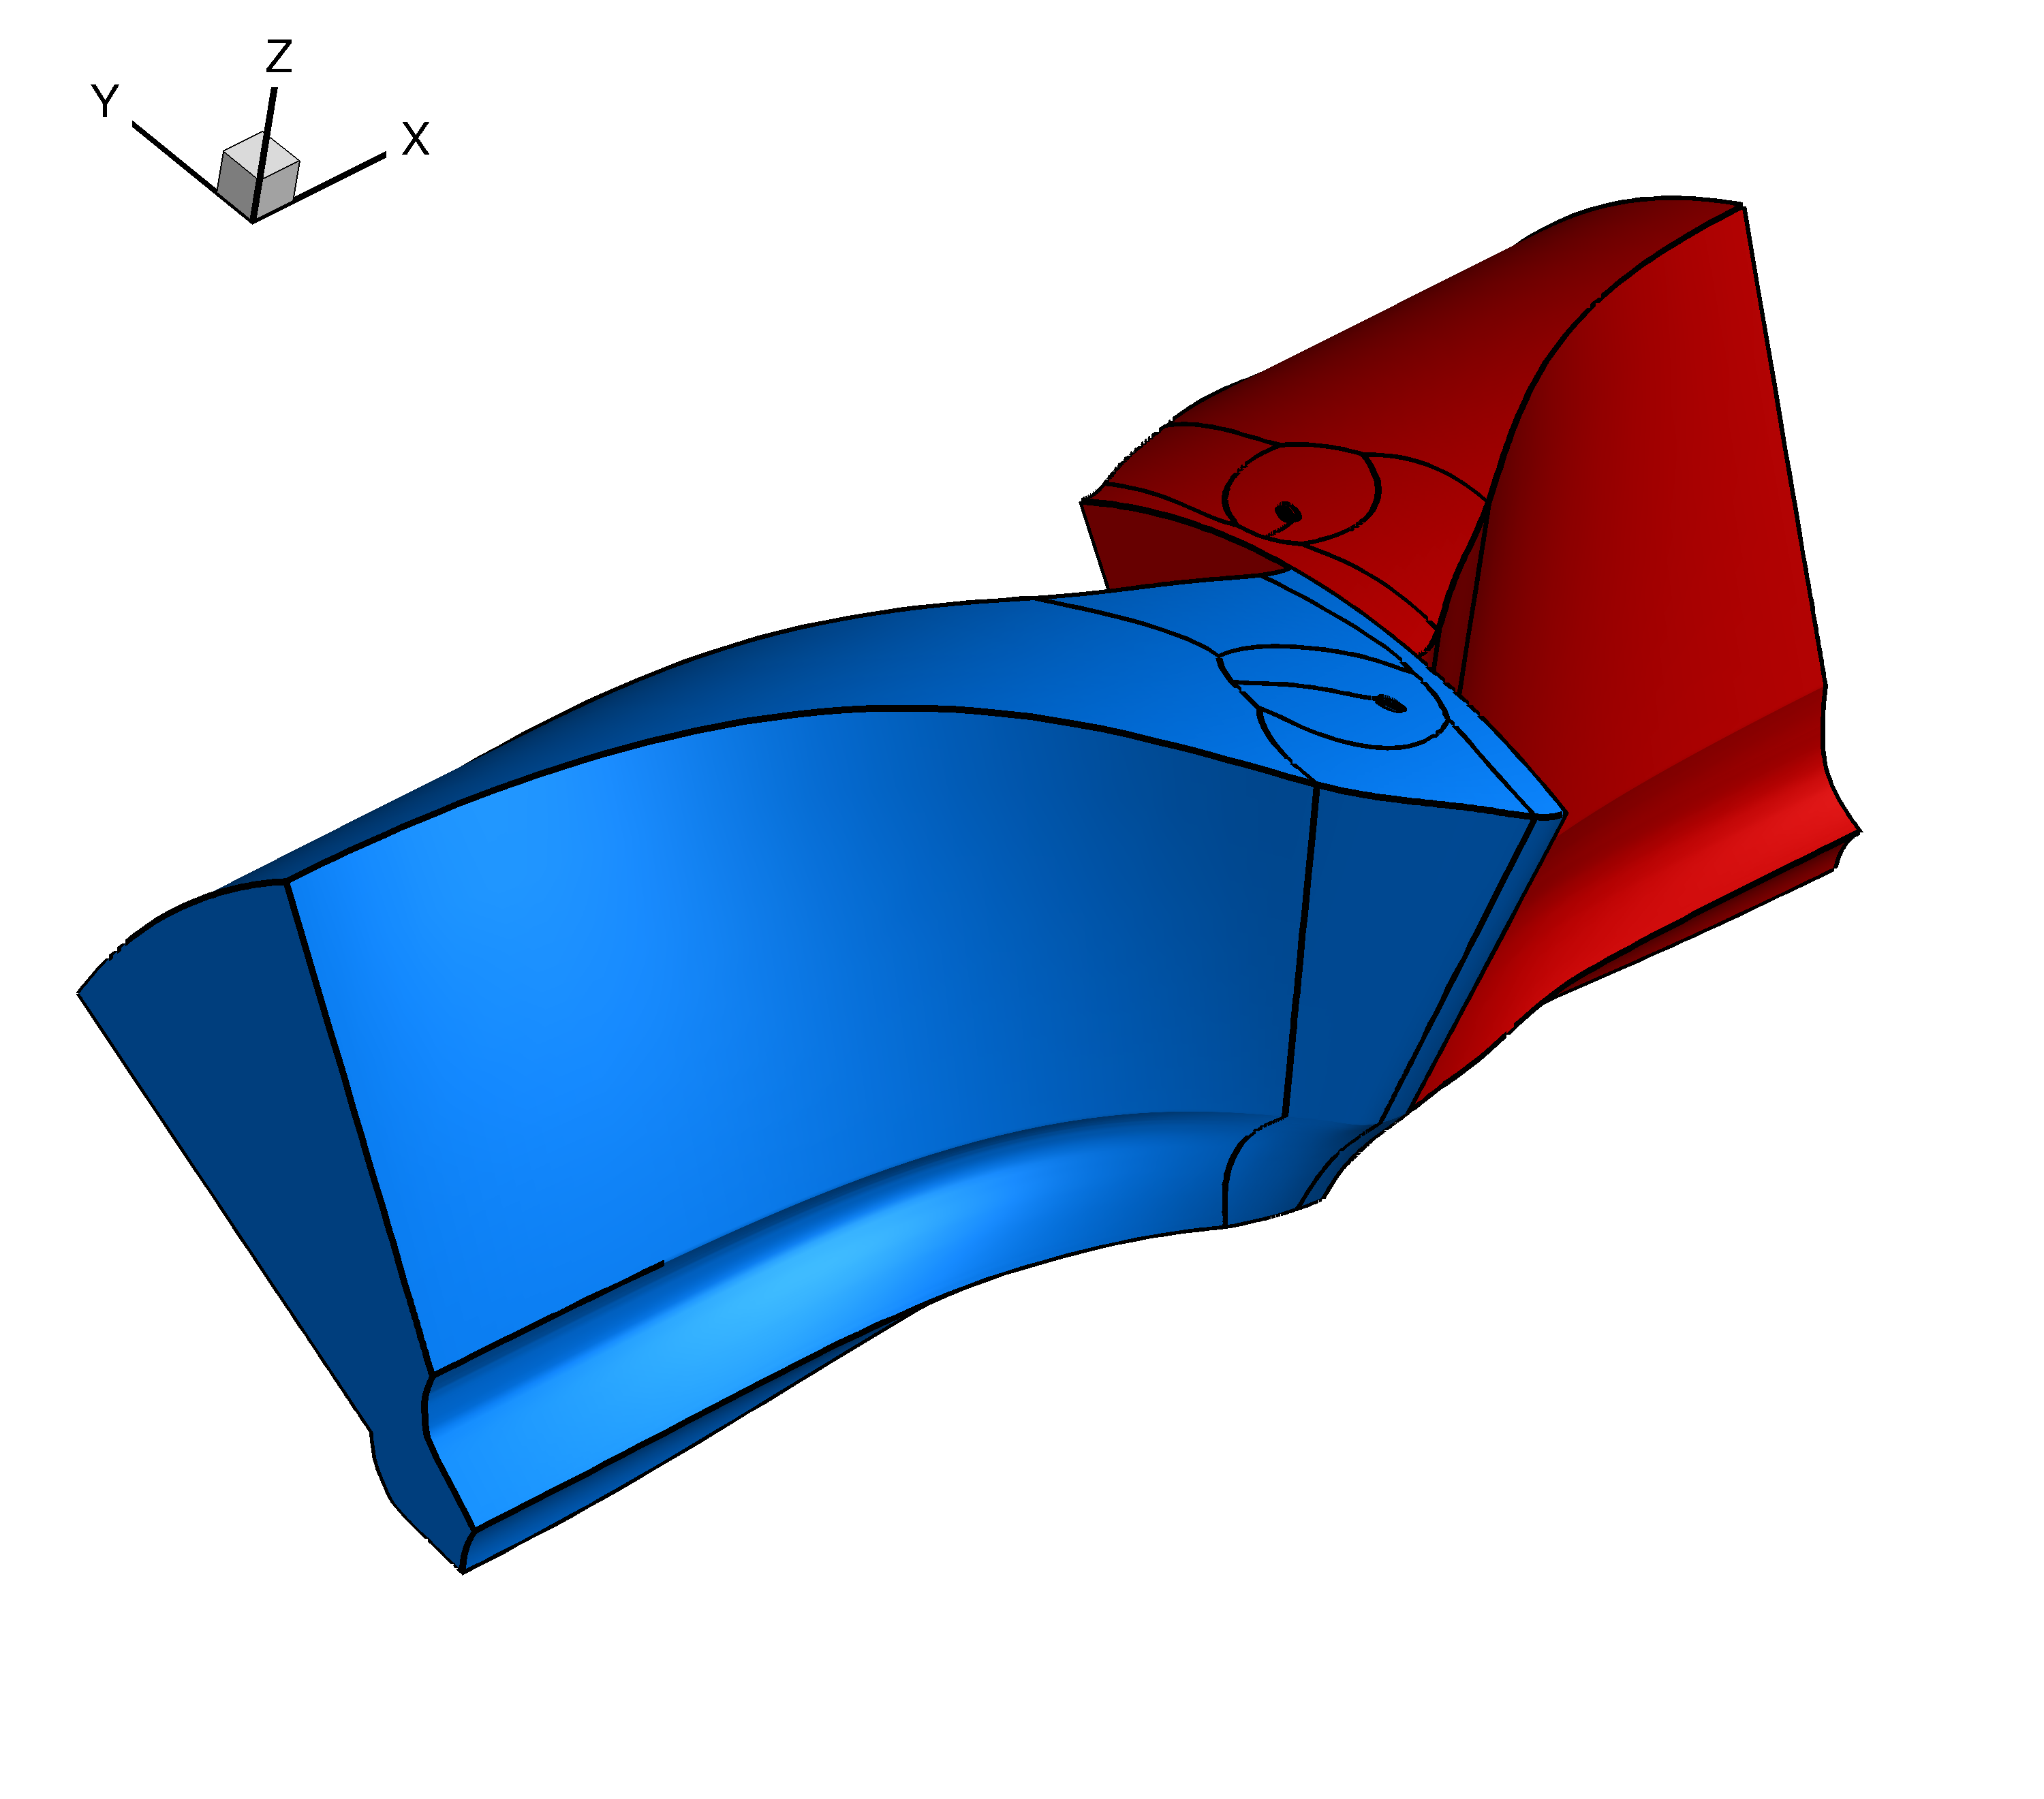
\includegraphics[height=.4\textwidth]{dream_mesh.png}}
  \subfigure[Detailed topology with number of grid points]{
    \label{fig:dream_ls_mesh}
    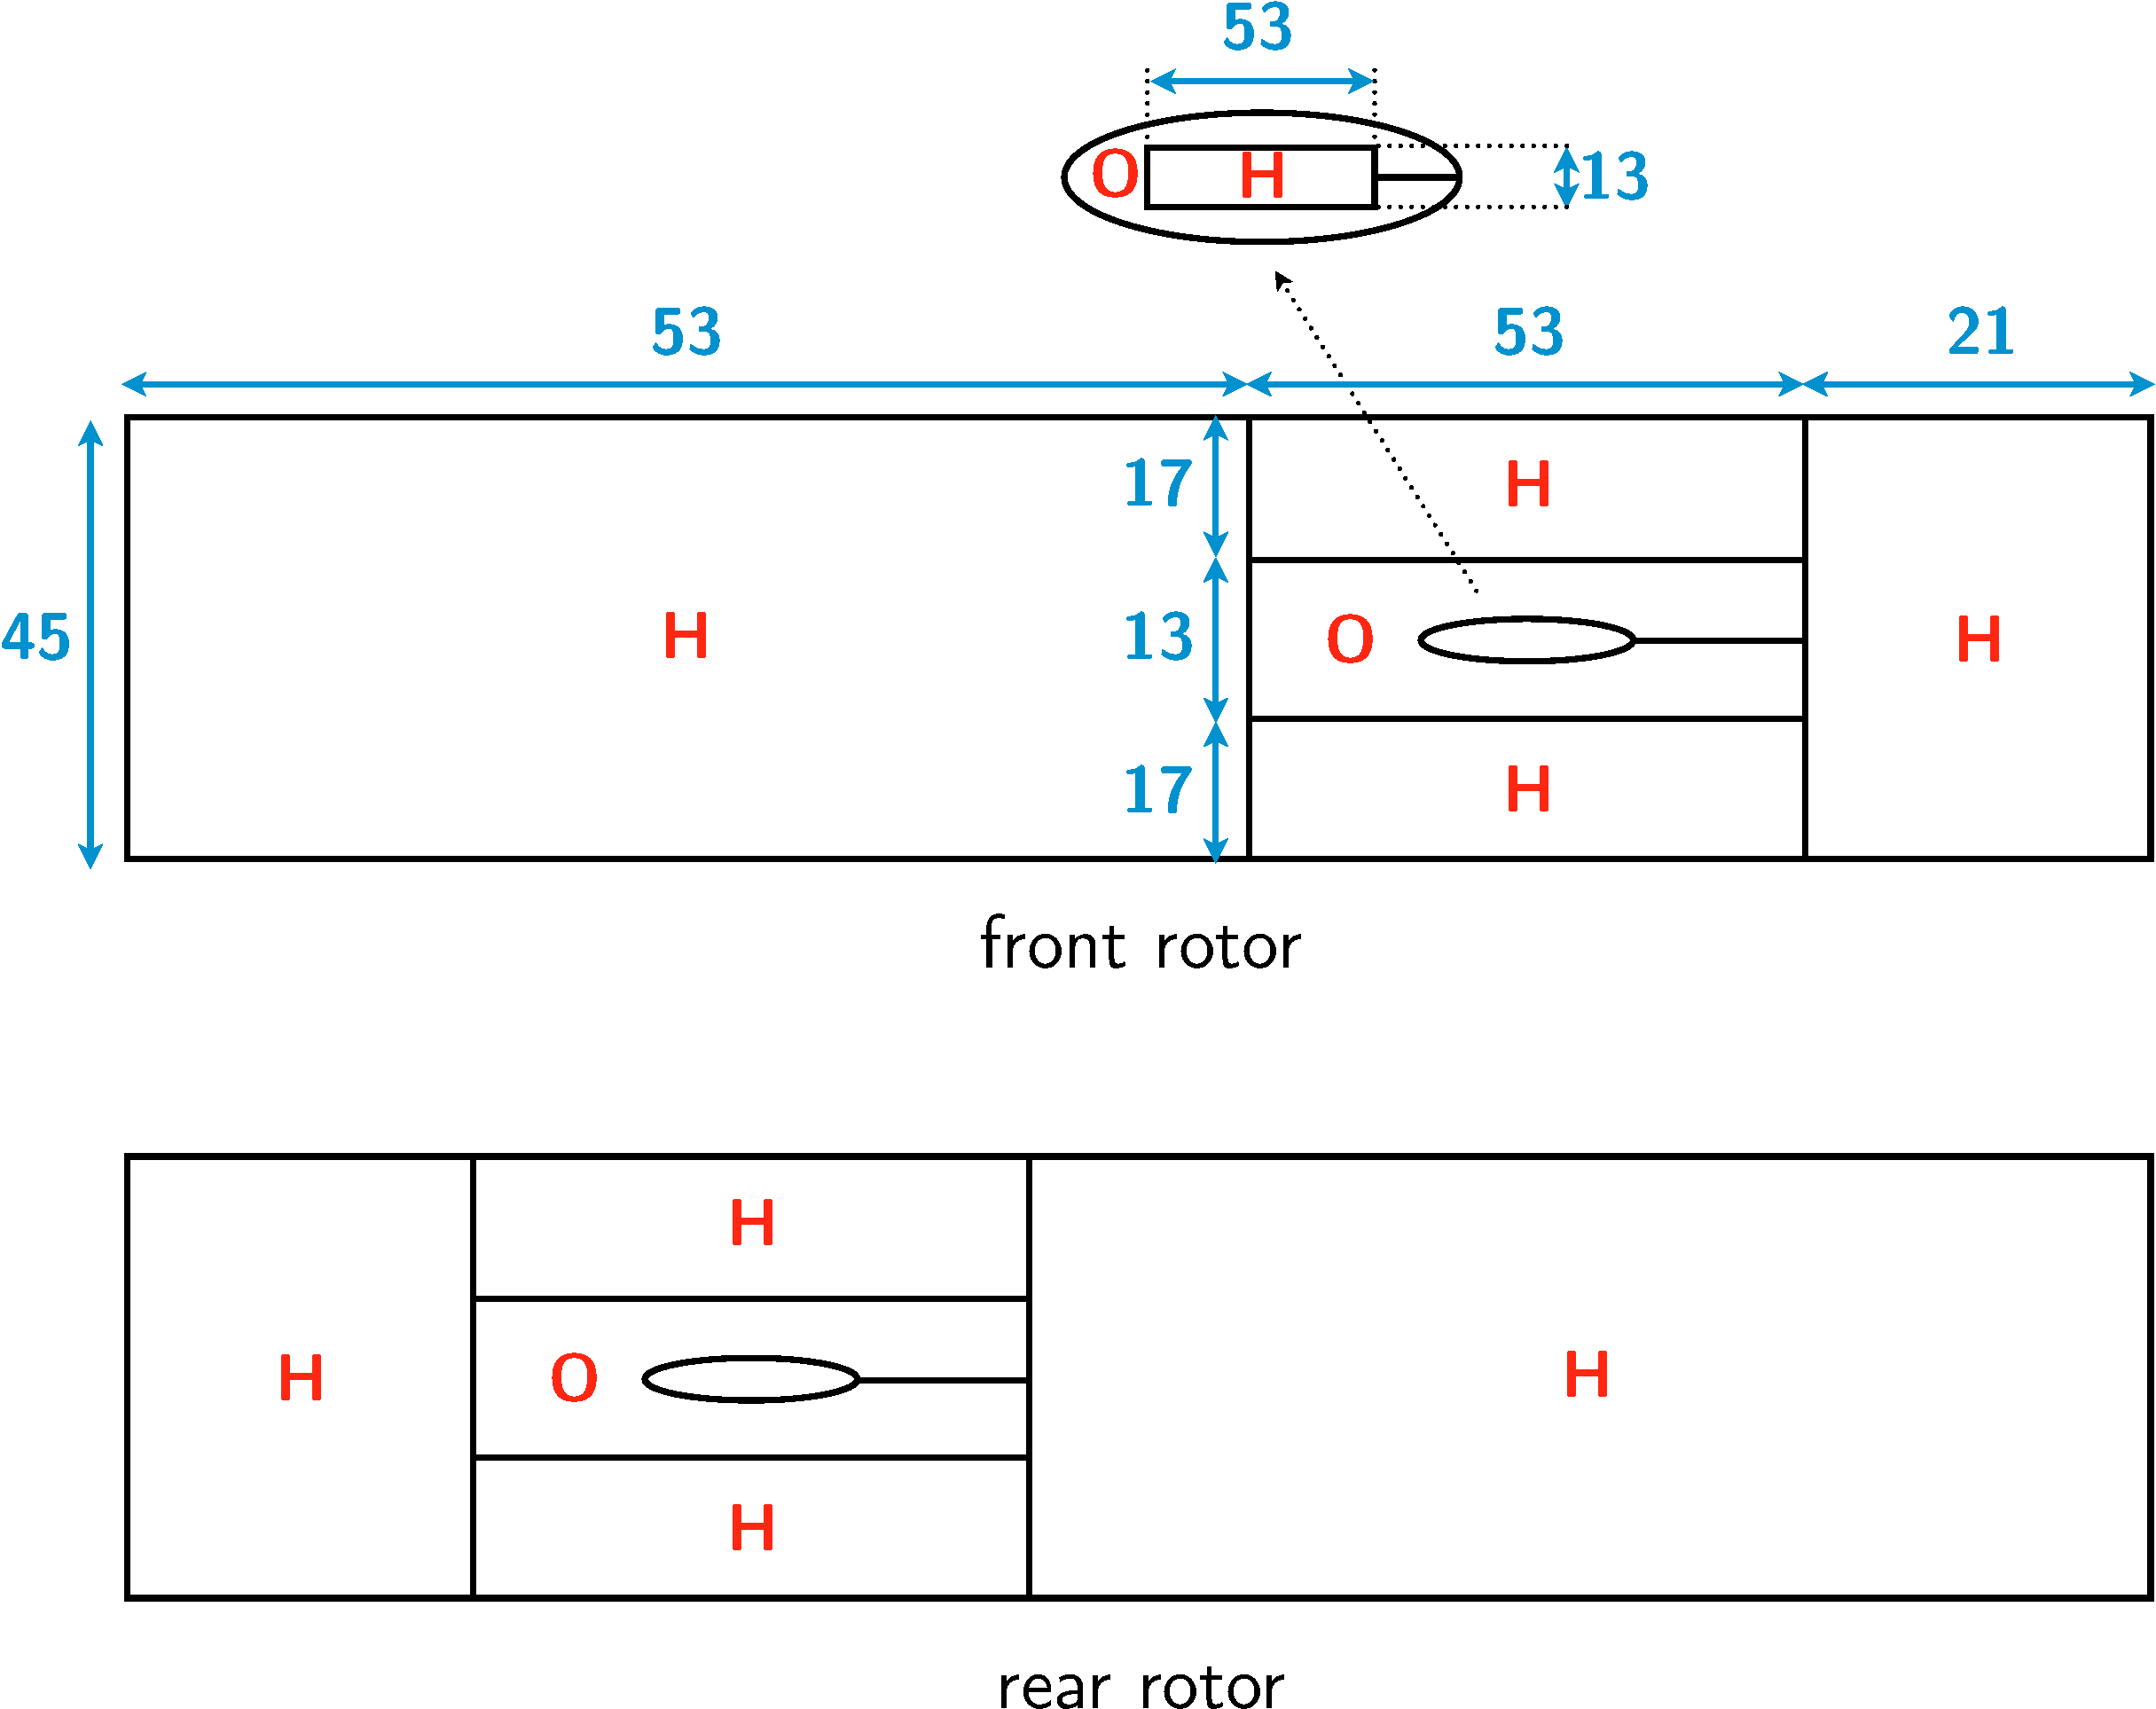
\includegraphics[height=.4\textwidth]{dream_ls_mesh.pdf}}
  \caption{Low-speed isolated configuration mesh topology.}
\end{figure}
The number of points is reported in 
Fig.~\ref{fig:dream_ls_mesh} for a blade-to-blade section. 
129~points discretize the blade, 45~the pitch and 181~the radial
extent. The same number of points is used for the front
and the rear rotors. These number of grid points are
classical inputs for steady RANS computations.

As a CROR is not shrouded, a sufficiently large
far-field domain is taken to ensure a minimum influence
of the far-field boundary conditions on the results.
The computational domain is shown in Fig.~\ref{fig:dream_farfield}.
The radial extent is $3D$ while the axial one is $3.5D$.
\citet{Peters2012} consider an axial extent of $7.5D$
with a radial extent of $4D$ while \citet{Zachariadis2011}
consider $2.5D$ and $3.6D$, respectively. We are thus in 
the mid-range of the values taken in the literature.
\begin{figure}[htb]
  \centering
  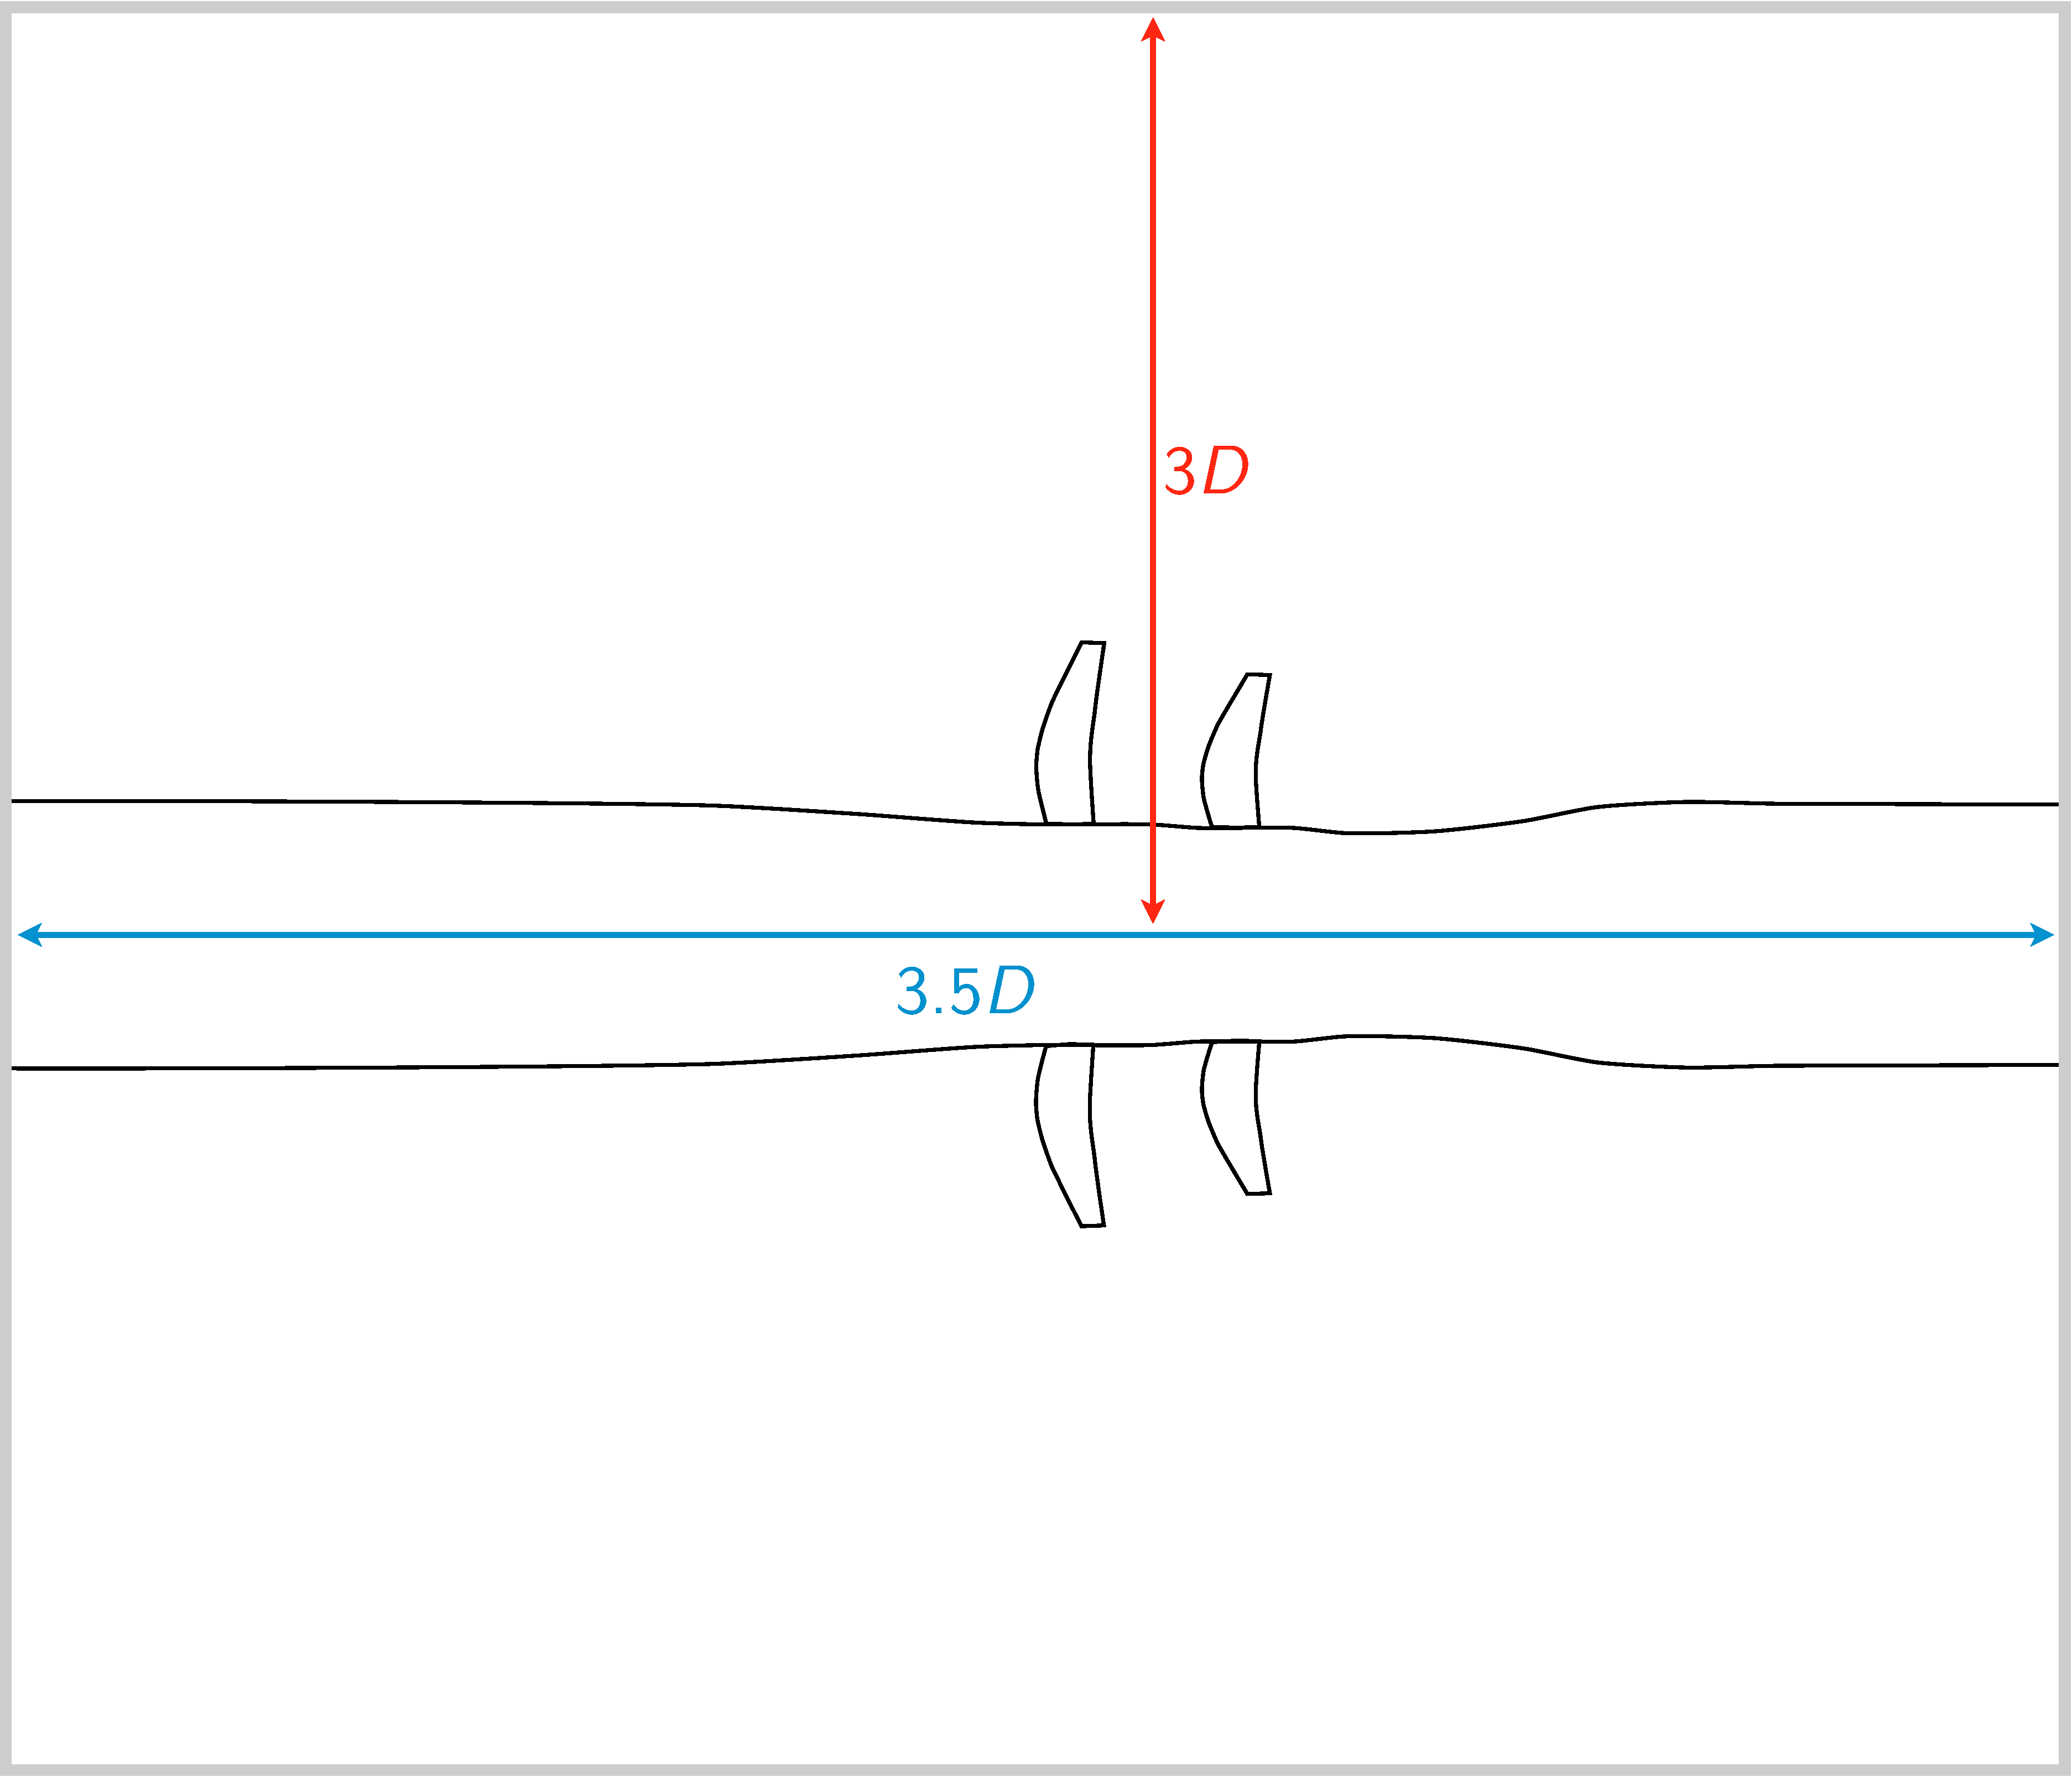
\includegraphics[width=.5\textwidth]{dream_farfield.pdf}
  \caption{Low-speed isolated configuration far-field domain and boundary conditions.}
  \label{fig:dream_farfield}
\end{figure}

As highlighted by underlined text in Fig.~\ref{fig:dream_farfield},
the boundary conditions used are: (i)~adiabatic walls
for the blades and the shroud (or spinner) and (ii)~constant
stagnation values used at the far-field.

Turbulence is modeled using the one-equation model of
\citet{Spalart1992}.  Roe's scheme~\cite{Roe1981} along with a 
second-order MUSL extrapolation 
is used to compute the convective fluxes.
The maximum CFL number is set to~10 for the steady 
computations and the HB simulations.

\subsection{Influence of the mesh discretization}
\label{sub:dream_ls_mesh_discretization}

To verify the quality of 

\subsection{Influence of the spatial discretization} % (fold)
\label{sub:dream_ls_spatial_discretization}

\begin{figure}[htb]
  \centering
  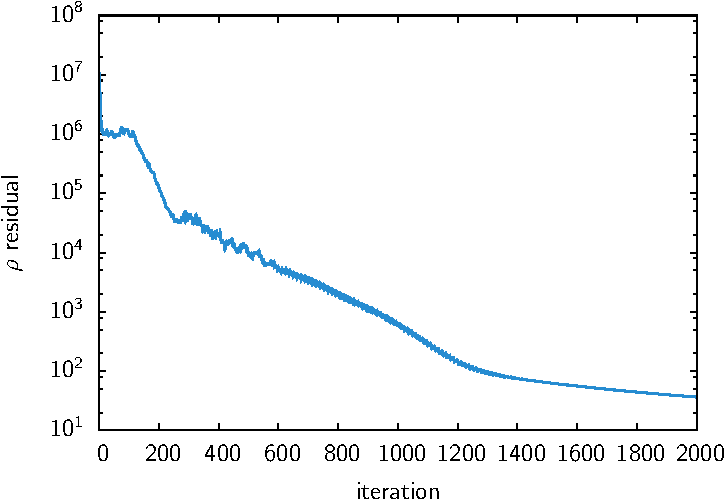
\includegraphics[width=.5\textwidth]{DREAM_LS_RESIDUALS_PPT.pdf}
  \caption{Convergence of the steady computations.}
  \label{fig:dream_operating_point}
\end{figure}

\begin{table}[htb]
  \ra{1.3} \centering
  \begin{tabular}{l|ccccccccc}
    \toprule
    \phantom{abdefghijk}& $C_{T_f}$ & $C_{P_f}$ & $\eta_f$ & $C_{T_r}$ & $C_{P_r}$ & $\eta_r$ & $C_T$ & $C_P$ & $\eta$ \\
    \midrule
    Roe 1 & $0.5135$ & $0.9762$ & $0.5568$ & $0.8421$ & $1.8895$ & $0.5242$ & $1.3555$ & $2.8657$ & $0.5353$ \\
    Roe 2 & $0.5637$ & $0.9941$ & $0.6002$ & $0.8664$ & $1.8613$ & $0.5475$ & $1.4301$ & $2.8554$ & $0.5659$ \\
    Roe 3 & $0.5684$ & $0.9937$ & $0.6054$ & $0.8715$ & $1.8618$ & $0.5506$ & $1.4398$ & $2.8555$ & $0.5697$ \\
    % JST $\kappa_4 = 0.016$ & $0.6128$ & $1.0647$ & $0.6093$ & $0.9514$ & $2.0401$ & $0.5485$ & $1.5642$ & $3.1048$ & $0.5694$ \\
    JST $\kappa_4 = 0.032$ & $0.5679$ & $0.9930$ & $0.6053$ & $0.8691$ & $1.8583$ & $0.5501$ & $1.4370$ & $2.8513$ & $0.5694$ \\
    JST $\kappa_4 = 0.064$ & $0.5666$ & $0.9921$ & $0.6045$ & $0.8669$ & $1.8558$ & $0.5495$ & $1.4335$ & $2.8478$ & $0.5687$ \\
    \bottomrule
  \end{tabular}
  \caption{Flight condition parameters.}
  \label{tab:dream_operating_point}
\end{table} 
